% ============================================================
%  CHAPITRE 3 — DONNÉES ET DÉVELOPPEMENT DU MODÈLE
% ============================================================
\chapter{Données et Développement du Modèle}
\label{chap:dataset}
\label{chap:modele}

\section{Introduction}

La qualité du dataset, la robustesse du prétraitement et la conception de l'architecture du réseau de neurones conditionnent directement les performances du système de segmentation. Avant qu'un modèle puisse distinguer une surface praticable d'un obstacle dangereux, les données doivent être validées, harmonisées, enrichies et optimisées pour le chargement. Ce chapitre présente le dataset utilisé, son exploration statistique, la chaîne de prétraitement appliquée, ainsi que le développement de l'architecture profonde (Attention U-Net) et du mécanisme de décision géométrique permettant de sélectionner automatiquement la meilleure zone d'atterrissage. Nous commençons par étudier la source de nos données en présentant les spécificités du jeu de données aériennes retenu.

\section{Présentation et exploration du dataset}
\label{sec:dataset-exploration}

Le projet s'appuie sur le \textbf{Graz Semantic Drone Dataset}~\cite{graz2015semantic}, une base publique de segmentation sémantique constituée d'images aériennes (\textit{vue top-down}) capturées entre 5 et 30 mètres d'altitude, couvrant des zones urbaines, périurbaines, des espaces naturels et des surfaces mixtes — des conditions représentatives d'un atterrissage d'urgence réel.

\begin{table}[!hb]
  \centering
  \caption{Caractéristiques du Graz Semantic Drone Dataset.}
  \label{tab:dataset-stats}
  \renewcommand{\arraystretch}{1.4}
  \begin{tabularx}{0.7\textwidth}{
    >{\bfseries\color{ENIADBlue}}l
    >{\centering\arraybackslash}X
  }
    \toprule
    \rowcolor{ENIADBlue!12}
    \textbf{Élément} & \textbf{Valeur} \\
    \midrule
    Nombre d'images / masques & 400 \\
    \rowcolor{ENIADLightBlue!20}
    Résolution originale & jusqu'à $6000 \times 4000$ px \\
    Résolution standardisée & $320 \times 320$ px \\
    \rowcolor{ENIADLightBlue!20}
    Classes sémantiques & 24 \\
    \bottomrule
  \end{tabularx}
\end{table}

Les 24 classes sémantiques sont regroupées en quatre catégories fonctionnelles :

\begin{table}[!hb]
  \centering
  \caption{Regroupement fonctionnel des 24 classes sémantiques.}
  \label{tab:classes}
  \renewcommand{\arraystretch}{1.4}
  \begin{tabularx}{0.95\textwidth}{
    >{\bfseries\color{ENIADBlue}}l
    >{\arraybackslash}X
  }
    \toprule
    \rowcolor{ENIADBlue!12}
    \textbf{Catégorie} & \textbf{Classes} \\
    \midrule
    Surfaces d'atterrissage potentielles & paved-area, grass, dirt, gravel \\
    \rowcolor{ENIADLightBlue!20}
    Obstacles critiques & person, dog, car, bicycle, water, pool \\
    Structures verticales & tree, bald-tree, vegetation, roof, wall, window, door, fence, fence-pole \\
    \rowcolor{ENIADLightBlue!20}
    Classes diverses & rocks, ar-marker, obstacle, conflicting, unlabeled \\
    \bottomrule
  \end{tabularx}
\end{table}

Pour le calcul du score de sécurité (décrit plus loin dans ce chapitre), ces classes sont regroupées en deux ensembles binaires : \textbf{Safe Classes} (paved-area, grass) et \textbf{Critical Obstacles} (person, dog, car, water).

\textbf{\textcolor{red}{Note :}} L'analyse exploratoire (EDA) révèle un déséquilibre marqué entre classes dominantes (\textit{paved-area}, \textit{grass}, \textit{roof}, \textit{tree}) et classes minoritaires (\textit{person}, \textit{dog}, \textit{bicycle}). Ce déséquilibre a directement motivé le choix de la Tversky Loss combinée à la Binary Cross Entropy, détaillé dans la suite de ce chapitre.

Pour exploiter ces classes de manière robuste malgré leur déséquilibre, les données brutes doivent subir une série de transformations et de normalisations que nous détaillons ci-après.

\section{Annotation et prétraitement}
\label{sec:pretraitement}

Chaque masque est stocké au format RGB, chaque couleur correspondant à une classe (ex. \texttt{[255,22,96]} $\rightarrow$ \textit{person}, \texttt{[0,102,0]} $\rightarrow$ \textit{grass}, \texttt{[128,64,128]} $\rightarrow$ \textit{paved-area}). Le pipeline de prétraitement, implémenté dans \texttt{DroneDataset} (\texttt{dataset.py}), applique successivement :

\begin{enumerate}[leftmargin=2em, itemsep=4pt, label=\textbf{\arabic*.}]
  \item \textbf{Validation} des paires image/masque (présence, correspondance des noms) via \texttt{\_validate\_coherence()} ;
  \item \textbf{Redimensionnement} à $320 \times 320$, avec interpolation linéaire pour les images et plus proche voisin pour les masques (afin de préserver les frontières de classes) ;
  \item \textbf{Normalisation} selon les statistiques ImageNet (moyenne $(0.485, 0.456, 0.406)$, écart-type $(0.229, 0.224, 0.225)$), nécessaire à la compatibilité avec l'encodeur EfficientNet-B0 pré-entraîné et à l'accélération de la convergence ;
  \item \textbf{Encodage LUT} des masques : chaque couleur RGB est convertie en un indice de classe via un hash \texttt{(R<<16)+(G<<8)+B}, réduisant fortement le temps de chargement CPU.
\end{enumerate}

\subsection{Augmentation des données (Data Augmentation)}
\label{subsec:data-augmentation}

Pour pallier la taille limitée de notre dataset (400 images) et prévenir tout risque de surapprentissage, un pipeline d'augmentation robuste basé sur la bibliothèque \texttt{Albumentations}~\cite{buslaev2020albumentations} a été conçu. Les transformations appliquées visent à simuler la diversité des scènes de vol réelles à travers quatre catégories fonctionnelles :

\begin{itemize}[leftmargin=1.8em, itemsep=4pt]
  \item \textbf{Robustesse géométrique} :
    \begin{itemize}[label=\textbullet, leftmargin=1.2em]
      \item \texttt{HorizontalFlip} ($p = 0.5$) et \texttt{VerticalFlip} ($p = 0.3$) : symétries axiales simulant des changements d'orientation de vol.
      \item \texttt{RandomRotate90} ($p = 0.5$) : rotation libre à $90^\circ$, idéale pour les prises de vue aériennes zénithales (\textit{top-down}) où l'orientation absolue n'a pas d'influence sémantique.
      \item \texttt{ShiftScaleRotate} ($p = 0.7$) : translation (limite $0.1$), échelle (limite $0.2$) et rotation (limite $30^\circ$) avec un mode de bordure par réflexion (\texttt{BORDER\_REFLECT\_101}) pour éviter les zones noires artificielles.
      \item \texttt{Perspective} ($p = 0.3$, échelle $0.04$ à $0.08$) : déformation de perspective simulant les inclinaisons angulaires de la caméra embarquée lors des mouvements de tangage et de roulis du drone.
    \end{itemize}
  \item \textbf{Robustesse photométrique} :
    \begin{itemize}[label=\textbullet, leftmargin=1.2em]
      \item \texttt{RandomBrightnessContrast} ($p = 0.6$, limite $0.3$) : ajustement aléatoire de la luminosité et du contraste pour faire face aux variations d'ensoleillement et d'exposition.
    \end{itemize}
  \item \textbf{Simulation de conditions météo et environnementales} :
    \begin{itemize}[label=\textbullet, leftmargin=1.2em]
      \item \texttt{RandomShadow} ($p = 0.3$) et \texttt{RandomFog} ($p = 0.2$) : ajout d'ombres portées et de brouillard artificiels, indispensables pour garantir la détection d'obstacles dans des environnements ombragés ou par temps couvert.
    \end{itemize}
  \item \textbf{Régularisation et normalisation} :
    \begin{itemize}[label=\textbullet, leftmargin=1.2em]
      \item \texttt{CoarseDropout} ($p = 0.3$, max. 8 trous de $32\times32$ px) : suppression aléatoire de rectangles de l'image (Cutout) pour forcer le modèle à apprendre des caractéristiques contextuelles globales et à tolérer les occlusions partielles d'obstacles.
      \item \texttt{Normalize} ($p = 1.0$) : normalisation finale centrée-réduite basée sur les statistiques ImageNet (moyenne $[0.485, 0.456, 0.406]$ et écart-type $[0.229, 0.224, 0.225]$) pour aligner les données avec les poids pré-entraînés du réseau.
    \end{itemize}
\end{itemize}

L'extrait de code suivant, tiré de notre script d'entraînement (annexe~\ref{sec:code-dataset-augmentation}), illustre la mise en œuvre de cette chaîne d'augmentation :

\begin{lstlisting}[language=Python, caption={Définition du pipeline d'augmentation des données via Albumentations.}]
train_transform = A.Compose([
    A.Resize(320, 320),
    A.HorizontalFlip(p=0.5),
    A.VerticalFlip(p=0.3),
    A.RandomRotate90(p=0.5),
    A.ShiftScaleRotate(
        shift_limit=0.1, scale_limit=0.2, rotate_limit=30,
        border_mode=cv2.BORDER_REFLECT_101, p=0.7
    ),
    A.Perspective(scale=(0.04, 0.08), p=0.3),
    A.RandomBrightnessContrast(brightness_limit=0.3, contrast_limit=0.3, p=0.6),
    A.CoarseDropout(
        max_holes=8, max_height=32, max_width=32,
        min_holes=1, fill_value=0, mask_fill_value=0, p=0.3
    ),
    A.Normalize(mean=(0.485, 0.456, 0.406), std=(0.229, 0.224, 0.225)),
    ToTensorV2(),
])
\end{lstlisting}

Après avoir préparé et enrichi ces images par cette chaîne d'augmentations, il convient de répartir équitablement le jeu de données pour l'entraînement et l'évaluation, ce qui fait l'objet de la section suivante.

\section{Séparation des données}
\label{sec:separation}

Le dataset a été réparti selon un ratio classique :

\begin{table}[!ht]
  \centering
  \caption{Répartition du dataset en ensembles d'entraînement, validation et test.}
  \label{tab:split}
  \renewcommand{\arraystretch}{1.4}
  \begin{tabularx}{0.65\textwidth}{
    >{\bfseries\color{ENIADBlue}}l
    >{\centering\arraybackslash}X
    >{\centering\arraybackslash}X
  }
    \toprule
    \rowcolor{ENIADBlue!12}
    \textbf{Ensemble} & \textbf{Ratio} & \textbf{Images} \\
    \midrule
    Entraînement & 70~\% & 280 \\
    \rowcolor{ENIADLightBlue!20}
    Validation & 15~\% & 60 \\
    Test & 15~\% & 60 \\
    \bottomrule
  \end{tabularx}
\end{table}

Une fois le dataset ainsi préparé, nettoyé et divisé en sous-ensembles d'apprentissage, de validation et de test, il peut alimenter la chaîne de traitement intelligente. La section suivante détaille le pipeline complet d'intelligence artificielle qui exploite ces données pour aboutir à la décision finale d'atterrissage sécurisé.

\section{Pipeline IA complet}
\label{sec:pipeline}

Le système transforme une scène aérienne brute en une décision d'atterrissage exploitable à travers une chaîne séquentielle organisée en quatre grandes phases thématiques (figure~\ref{fig:pipeline-global}) : la phase d'acquisition (bleue, englobant la capture vidéo de la caméra et le prétraitement d'image), la phase de segmentation et décision (orange, comprenant l'inférence du modèle U-Net pour la génération du masque sémantique binaire et la sélection de zone par l'analyse des zones sûres), la phase de guidage et contrôle (verte, associant la machine d'états pour la gestion des états, le Guidance Controller et le Flight Controller assurant les commandes bas niveau), et enfin la phase de communication et d'actionnement (grise, regroupant le protocole MAVLink pour la communication standard, le firmware de vol PX4/ArduPilot et l'exécution physique sur le drone).

\begin{figure}[!ht]
  \centering
  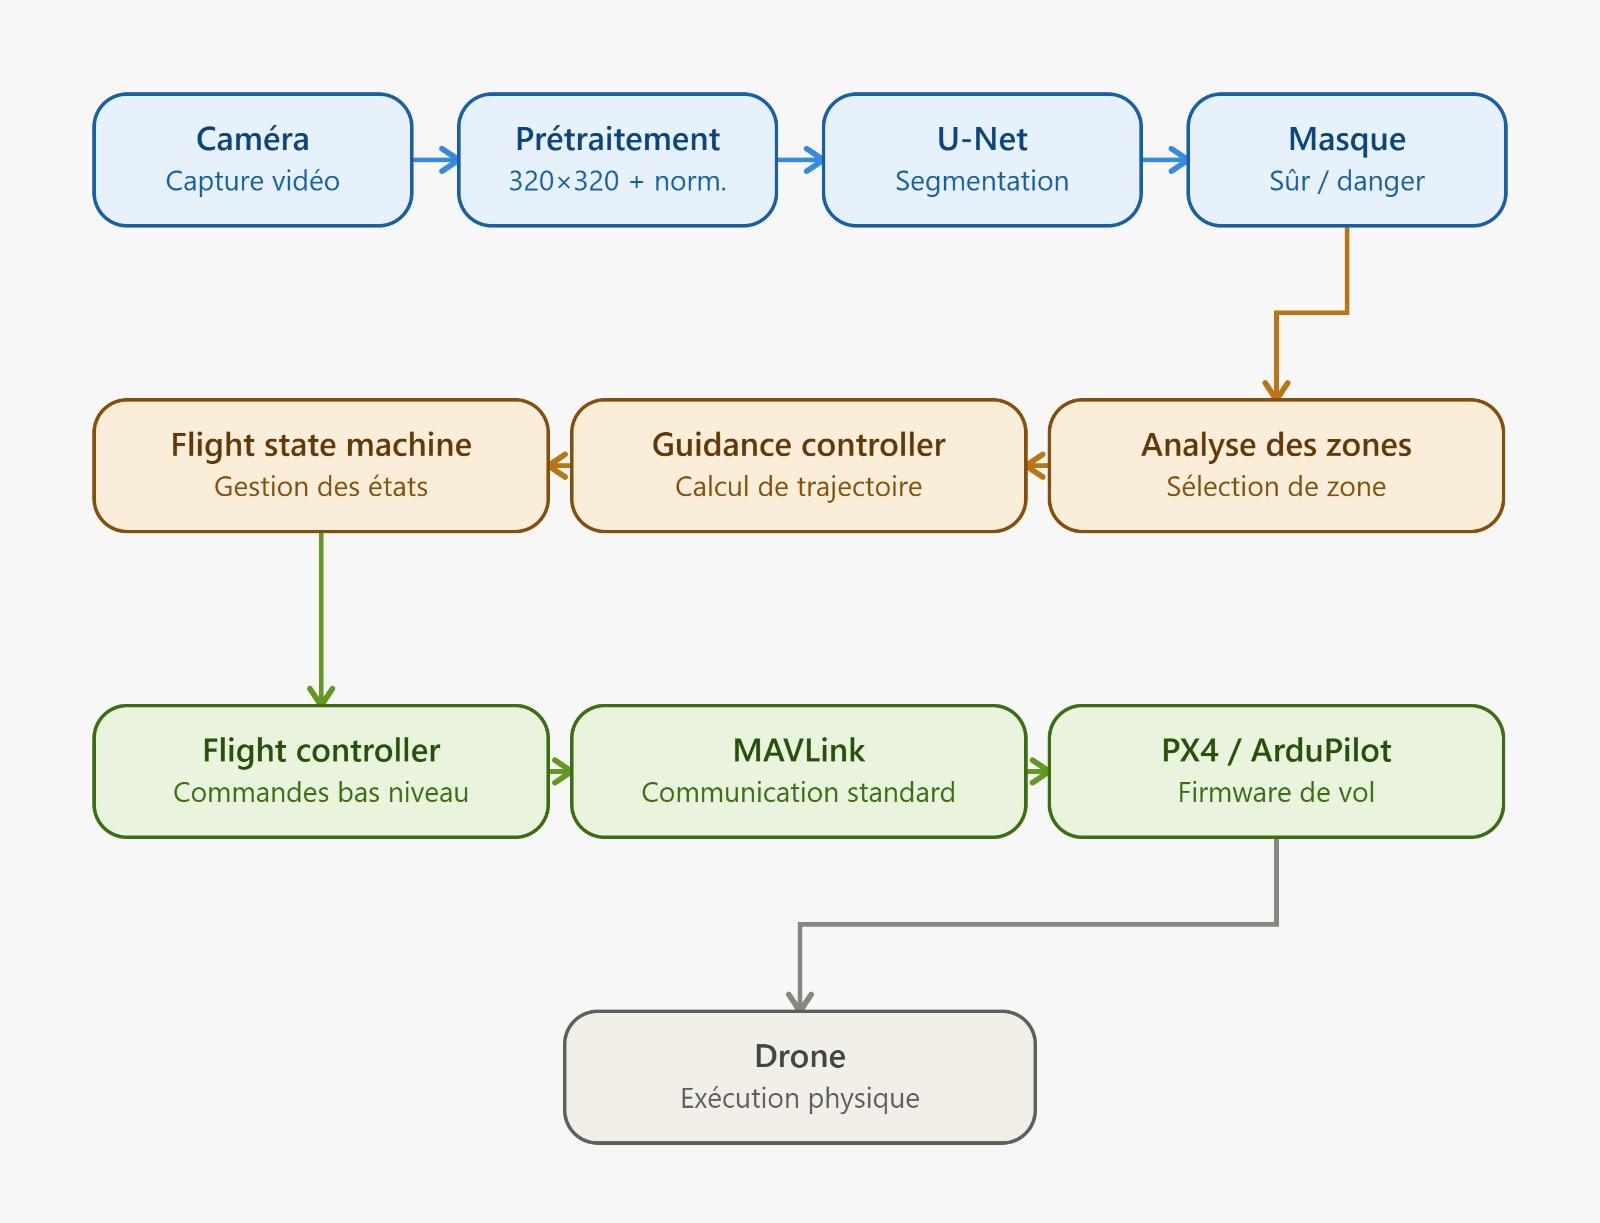
\includegraphics[width=0.8\textwidth,keepaspectratio]{1.jpeg}
  \caption{Pipeline global du système d'atterrissage autonome, depuis la capture caméra jusqu'à l'exécution physique sur le drone via PX4/ArduPilot.}
  \label{fig:pipeline-global}
\end{figure}

À partir du masque sémantique binaire, le système calcule une Distance Transform entre chaque région praticable et les obstacles détectés, puis évalue un score de sécurité pour identifier automatiquement la zone offrant le meilleur niveau de sûreté. Les étapes de ce traitement, depuis la prédiction du masque jusqu'à l'extraction de la zone la plus sûre, sont illustrées dans la figure~\ref{fig:best-landing-point}.

\begin{figure}[!hb]
  \centering
  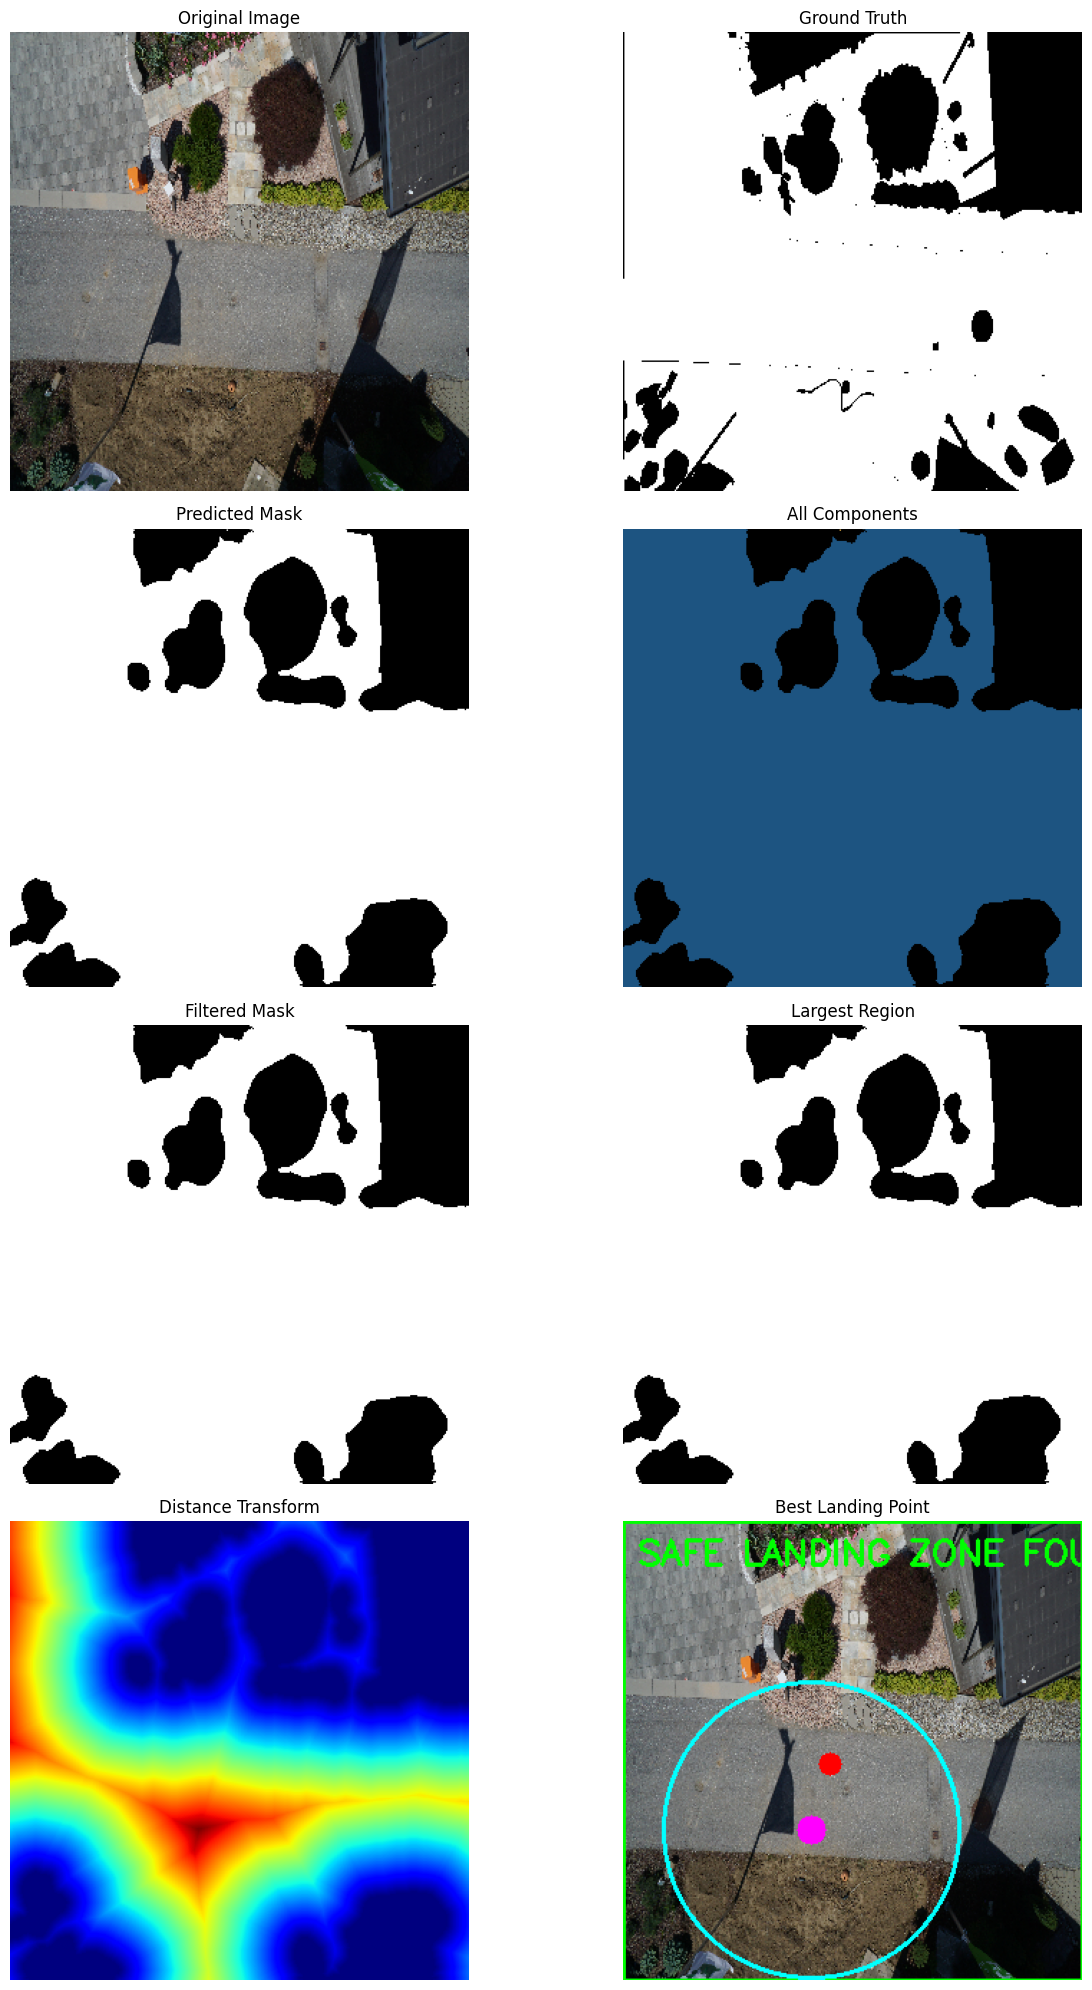
\includegraphics[width=0.5\textwidth,keepaspectratio]{assets/model/best_landing_point.png}
  \caption{Étapes de détection de la zone d'atterrissage la plus sûre (\textit{best area}) : image originale, vérité terrain, masque prédit, composantes connexes, masque filtré par aire minimale ($5000$ px), sélection de la plus grande région, application de la Distance Transform et localisation du point d'atterrissage optimal.}
  \label{fig:best-landing-point}
\end{figure}

Ce pipeline décisionnel repose au premier plan sur les algorithmes de guidage et de pilotage décrits dans la section suivante.

\section{Contrôleur de guidage et machine d'états}
\label{sec:guidage-state-machine}

Une fois la zone d'atterrissage optimale identifiée par le pipeline de vision, les coordonnées du point cible doivent être converties en commandes de vol pour guider le drone de manière autonome. Cette logique de pilotage de haut niveau associe un contrôleur de guidage géométrique et une machine d'états de vol.

\subsection{Sélection du point d'atterrissage optimal}

Le module d'analyse extrait les composantes connexes du masque de pixels sûrs. Les zones dont l'aire est inférieure à un seuil critique de sécurité ($5000$ pixels dans notre implémentation) sont exclues afin d'éviter tout atterrissage dans des clairières exiguës ou à proximité immédiate d'obstacles. Sur la plus grande composante connexe retenue, la Distance Transform euclidienne est calculée. L'algorithme recherche ensuite le point maximisant cette distance via \texttt{cv2.minMaxLoc()}, ce qui correspond au centre du plus grand cercle exempt d'obstacles inscrit dans la zone. Ce point, qui garantit la plus grande marge de sécurité physique par rapport aux menaces environnantes, est alors transmis au module de guidage.

\subsection{Contrôleur de guidage géométrique}

Le contrôleur de guidage, dont l'implémentation est détaillée à l'annexe~\ref{sec:code-guidage-machine}, calcule à chaque cycle l'erreur horizontale ($dx$) et verticale ($dy$) entre le centre de l'image (représentant la position actuelle du drone en vol stationnaire zénithal) et les coordonnées du point cible :
\begin{equation}
  dx = X_{\text{cible}} - X_{\text{centre}}, \quad dy = Y_{\text{cible}} - Y_{\text{centre}}
\end{equation}
La distance euclidienne $D = \sqrt{dx^2 + dy^2}$ et l'angle de gisement (\textit{heading}) $\theta = \arctan2(dy, dx)$ sont calculés pour orienter le drone. Une zone de tolérance de $\pm 10$ pixels est appliquée : si l'écart dépasse ce seuil, le contrôleur émet des commandes directionnelles discrètes (\texttt{MOVE LEFT}, \texttt{MOVE RIGHT}, \texttt{MOVE FORWARD}, \texttt{MOVE BACKWARD}), sinon il passe en commande stationnaire (\texttt{HOLD}) et active le signal de centrage.

\subsection{Machine d'états de vol}

Pour orchestrer le comportement dynamique du drone en situation d'urgence, une machine d'états à trois modes est définie (figure~\ref{fig:guidance-visualisation}) :
\begin{itemize}[leftmargin=1.8em, itemsep=4pt]
  \item \textbf{SEARCHING} : Le drone balaie la zone à la recherche d'une surface praticable d'une aire minimale requise. Dès qu'une zone valide est détectée et autorisée par le score de sécurité, le système bascule vers l'état \textbf{GUIDING}.
  \item \textbf{GUIDING} : Le drone applique les commandes générées par le contrôleur de guidage pour se déplacer en translation vers le point d'atterrissage optimal. Si la zone devient indisponible ou obstruée, il retourne à l'état \textbf{SEARCHING} ; si le drone parvient à se centrer au-dessus de la cible dans la tolérance admise, il transite vers l'état \textbf{LANDING}.
  \item \textbf{LANDING} : Le drone déclenche sa descente verticale finale. Si un obstacle surgit durant la descente, la machine d'états interrompt la procédure et réactive l'état \textbf{SEARCHING} pour trouver une zone alternative.
\end{itemize}

\begin{figure}[!hb]
  \centering
  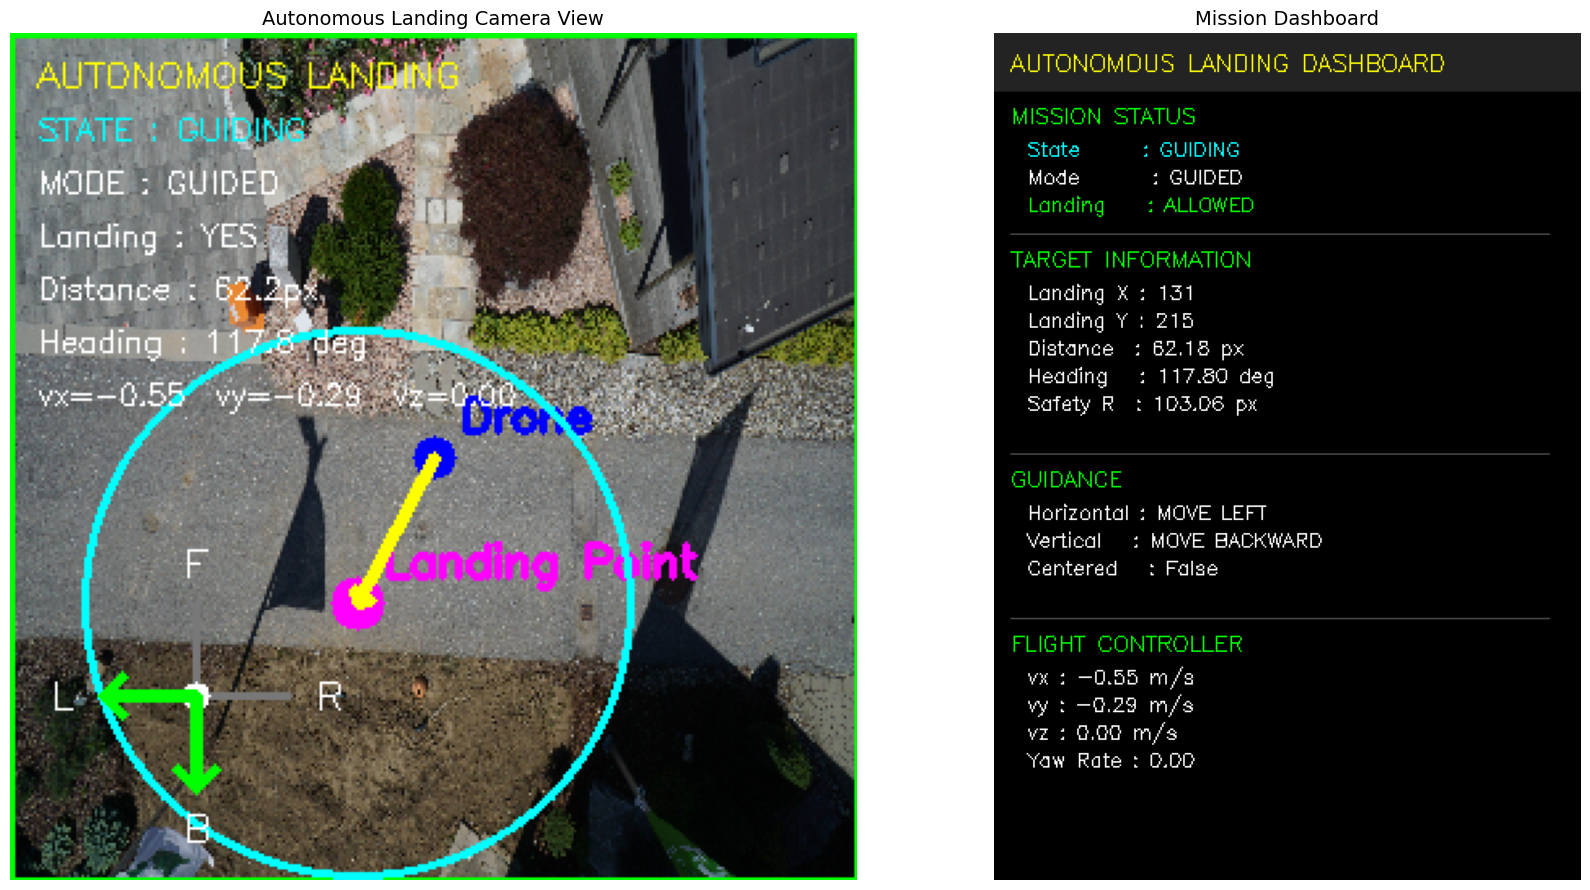
\includegraphics[width=0.55\textwidth,keepaspectratio]{assets/model/guidance_visualisation_v2.png}
  \caption{Visualisation de guidage finale (drone centré sur la zone d'atterrissage sélectionnée).}
  \label{fig:guidance-visualisation}
\end{figure}

\subsection{Contrôleur de vol (Flight Controller)}
\label{subsec:flight-controller}

Le module final de la chaîne de décision est le contrôleur de vol (\textit{Flight Controller}). Ce module sert de couche d'adaptation logique entre les commandes géométriques de haut niveau et le pilotage bas niveau du drone.

Concrètement, le contrôleur de vol reçoit à chaque itération l'état courant de la machine d'états de vol (\texttt{SEARCHING}, \texttt{GUIDING} ou \texttt{LANDING}) ainsi que les consignes directionnelles calculées par le contrôleur de guidage (\texttt{MOVE LEFT}, \texttt{MOVE RIGHT}, \texttt{MOVE FORWARD}, \texttt{MOVE BACKWARD} ou \texttt{HOLD}). Son rôle est d'interpréter ces données pour générer des consignes de vitesses tridimensionnelles ($v_x$, $v_y$, $v_z$) et de taux de lacet (\textit{yaw rate}) adaptées aux attentes de l'autopilote :
\begin{itemize}[leftmargin=1.8em, itemsep=4pt]
  \item En état \textbf{SEARCHING} : Les vitesses de translation sont maintenues nulles, et le drone effectue un balayage rotatif lent pour acquérir de nouvelles images.
  \item En état \textbf{GUIDING} : Les commandes discrètes du guidage (ex. \texttt{MOVE FORWARD}) sont converties en vitesses de translation proportionnelles (ex. $v_x = 0.5$ m/s), tout en maintenant l'altitude constante.
  \item En état \textbf{LANDING} : Les vitesses horizontales sont annulées, et une vitesse verticale de descente contrôlée ($v_z = -0.25$ m/s) est commandée jusqu'au toucher du sol.
\end{itemize}

Ces consignes sont conçues pour être encapsulées sous forme de messages du protocole \textit{MAVLink} afin d'être transmises au micrologiciel de l'autopilote (comme PX4 ou ArduPilot) via une liaison série ou réseau. Dans le cadre de ce projet, ce module de commande de vol a été implémenté et évalué de façon logicielle hors ligne (sur flux d'images statiques de test), jetant les bases algorithmiques requises pour une validation future sur drone physique. L'implémentation complète de cette interface logique et de la machine de vol est fournie à l'annexe~\ref{sec:code-guidage-machine}.

Ce pipeline de guidage et de contrôle de vol complète notre système intelligent en aval de la segmentation sémantique. L'architecture profonde qui permet d'obtenir le masque sémantique de départ est détaillée dans la section suivante.

\section{Architecture du modèle}
\label{sec:architecture-modele}

Le réseau suit le principe de l'architecture Attention U-Net~\cite{oktay2018attention} enrichi d'un encodeur EfficientNet-B0~\cite{tan2019efficientnet} pré-entraîné et de connexions résiduelles.

\subsection{Encodeur — EfficientNet-B0}

EfficientNet-B0 extrait progressivement les caractéristiques de l'image par niveaux successifs, la résolution spatiale diminuant à mesure que la richesse sémantique augmente :

\begin{table}[!ht]
  \centering
  \caption{Niveaux de l'encodeur EfficientNet-B0.}
  \label{tab:encodeur}
  \renewcommand{\arraystretch}{1.4}
  \begin{tabularx}{0.65\textwidth}{
    >{\bfseries\color{ENIADBlue}}c
    >{\centering\arraybackslash}X
    >{\centering\arraybackslash}X
  }
    \toprule
    \rowcolor{ENIADBlue!12}
    \textbf{Niveau} & \textbf{Canaux} & \textbf{Taille} \\
    \midrule
    Bloc 1 & 16 & $160\times160$ \\
    \rowcolor{ENIADLightBlue!20}
    Bloc 2 & 24 & $80\times80$ \\
    Bloc 3 & 40 & $40\times40$ \\
    \rowcolor{ENIADLightBlue!20}
    Bloc 4 & 112 & $20\times20$ \\
    Bloc 5 & 320 & $10\times10$ \\
    \bottomrule
  \end{tabularx}
\end{table}

\subsection{Skip connections}

Pour limiter la perte d'informations fines lors de la compression, des connexions résiduelles (skip connections) transfèrent directement les cartes de caractéristiques haute résolution de l'encodeur vers le décodeur, améliorant la reconstruction spatiale et la précision des contours.

\subsection{Sortie}

Une convolution finale $1\times1$ réduit les caractéristiques à 1 seule carte, convertie en probabilités par une fonction Sigmoïde afin d'obtenir un masque binaire final indiquant si la zone est praticable (SAFE) ou non (UNSAFE). La définition de cette architecture étant posée, son apprentissage nécessite de configurer des hyperparamètres précis, détaillés dans la section suivante.

\section{Hyperparamètres et configuration d'entraînement}
\label{sec:hyperparams}

\begin{table}[!ht]
  \centering
  \caption{Hyperparamètres d'entraînement du modèle.}
  \label{tab:hyperparams}
  \renewcommand{\arraystretch}{1.4}
  \begin{tabularx}{0.75\textwidth}{
    >{\bfseries\color{ENIADBlue}}l
    >{\centering\arraybackslash}X
  }
    \toprule
    \rowcolor{ENIADBlue!12}
    \textbf{Paramètre} & \textbf{Valeur} \\
    \midrule
    Époques max. & 150 (Early Stopping à 128) \\
    \rowcolor{ENIADLightBlue!20}
    Batch Size & 8 \\
    Learning Rate & 0.0003 \\
    \rowcolor{ENIADLightBlue!20}
    Optimiseur & AdamW~\cite{loshchilov2019adamw} \\
    Weight Decay & 0.0001 \\
    \rowcolor{ENIADLightBlue!20}
    Scheduler & Cosine Annealing (avec redémarrages)~\cite{loshchilov2017sgdr} \\
    Mixed Precision & Activé (AMP)~\cite{micikevicius2018mixed} \\
    \rowcolor{ENIADLightBlue!20}
    Early Stopping & Activé (patience = 15) \\
    Patience LR Scheduler & 5 \\
    \rowcolor{ENIADLightBlue!20}
    Seed & 42 \\
    \bottomrule
  \end{tabularx}
\end{table}

Pour assurer la clarté et la reproductibilité de notre configuration, la définition et le rôle de chaque hyperparamètre configuré dans le tableau~\ref{tab:hyperparams} sont détaillés ci-après :
\begin{itemize}[leftmargin=1.8em, itemsep=6pt]
  \item \textbf{Époques max. et Early Stopping} : L'entraînement est planifié sur un maximum de $150$ époques. Pour prévenir le surapprentissage (\textit{overfitting}) et optimiser le temps de calcul, un mécanisme d'\textit{Early Stopping} surveille la perte de validation. Si celle-ci ne s'améliore plus sur $15$ époques consécutives (patience $= 15$), l'entraînement s'arrête. Dans notre cas, il s'est interrompu à l'époque $128$, le meilleur modèle ayant été obtenu et sauvegardé à l'époque $113$.
  \item \textbf{Batch Size} : Fixé à $8$, ce paramètre définit le nombre d'images traitées simultanément avant d'effectuer une rétropropagation du gradient. Ce choix modeste est imposé par les limites de mémoire vidéo (VRAM) du GPU lors du traitement de grandes résolutions ($320\times320$ pixels) à travers une architecture à double branche (encodeur-décodeur).
  \item \textbf{Learning Rate (Taux d'apprentissage)} : Réglé à $3\times10^{-4}$ ($0.0003$), il détermine l'amplitude de mise à jour des poids à chaque pas d'optimisation, garantissant un apprentissage stable et progressif.
  \item \textbf{Optimiseur AdamW}~\cite{loshchilov2019adamw} : Cette variante de l'optimiseur Adam classique découple la pénalité de poids (\textit{Weight Decay}) de la mise à jour des gradients adaptatifs, améliorant la généralisation sur de nouvelles images. Il a été sélectionné pour sa convergence rapide et stable, particulièrement adaptée pour ajuster finement les poids d'un encodeur pré-entraîné comme EfficientNet-B0.
  \item \textbf{Weight Decay} : Fixé à $10^{-4}$ ($0.0001$), il s'agit d'une régularisation L2 qui pénalise les poids trop élevés afin de régulariser le réseau et de limiter le surapprentissage.
  \item \textbf{Scheduler (Cosine Annealing avec redémarrages à chaud)}~\cite{loshchilov2017sgdr} : Un \textit{scheduler} fait varier le taux d'apprentissage au fil des époques plutôt que de le maintenir fixe. Le mécanisme \textit{Cosine Annealing} diminue le taux d'apprentissage selon une fonction cosinusoïdale. Les redémarrages à chaud (\textit{warm restarts}) réinitialisent périodiquement le taux d'apprentissage à son maximum (période initiale $T_0 = 20$ époques) pour aider le modèle à s'extraire de minima locaux d'optimisation.
  \item \textbf{Mixed Precision (AMP)}~\cite{micikevicius2018mixed} : L'entraînement en précision mixte (\textit{Automatic Mixed Precision}) effectue une partie des opérations matricielles en précision FP16 (plutôt que FP32). Cela réduit l'utilisation de la VRAM GPU et accélère l'inférence pendant l'apprentissage sans dégradation significative des performances.
  \item \textbf{Graine aléatoire (Seed)} : Fixée à $42$ et synchronisée entre Python, NumPy et PyTorch, elle garantit la reproductibilité des partitions de données et de l'initialisation des poids du modèle.
\end{itemize}

Le succès de cet entraînement dépend également de la fonction de coût choisie pour guider la correction du réseau, que nous décrivons ci-après.

\section{Fonction de coût}
\label{sec:loss}

La fonction de coût désigne l'écart entre la prédiction du réseau et la vérité terrain à chaque itération. Dans le contexte d'une segmentation binaire aérienne, la Binary Cross Entropy (BCE) Loss seule peut souffrir du déséquilibre entre les pixels des zones sûres et ceux des obstacles. La Tversky Loss~\cite{salehi2017tversky}, qui généralise la Dice Loss~\cite{milletari2016vnet}, compense cette limite en pénalisant plus lourdement les faux négatifs pour assurer la sécurité de l'atterrissage.

\begin{table}[!ht]
  \centering
  \caption{Comparaison des fonctions de coût.}
  \label{tab:loss}
  \renewcommand{\arraystretch}{1.4}
  \begin{tabularx}{0.9\textwidth}{
    >{\bfseries\color{ENIADBlue}}l
    >{\centering\arraybackslash}X
    >{\centering\arraybackslash}X
  }
    \toprule
    \rowcolor{ENIADBlue!12}
    & \textbf{BCE Loss} & \textbf{Tversky Loss} \\
    \midrule
    Avantage principal & Convergence stable & Robuste au déséquilibre, évite les faux négatifs \\
    \rowcolor{ENIADLightBlue!20}
    Limite principale & Ignore le déséquilibre & Instable seule \\
    \bottomrule
  \end{tabularx}
\end{table}

Le modèle final combine donc les deux fonctions à parts égales (poids $0.5 / 0.5$), offrant simultanément la stabilité de la BCE et la sensibilité aux faux négatifs de la Tversky Loss (avec $\alpha=0.3$ pour les faux positifs et $\beta=0.7$ pour pénaliser plus fortement les faux négatifs) sur les zones d'atterrissage sécurisées. Pour accélérer cet apprentissage et garantir sa robustesse matérielle, plusieurs optimisations techniques complémentaires ont été intégrées au pipeline d'entraînement.

\section{Optimisations du modèle}
\label{sec:optimisations}

\begin{table}[!ht]
  \centering
  \caption{Optimisations techniques intégrées à l'entraînement.}
  \label{tab:optimisations}
  \renewcommand{\arraystretch}{1.4}
  \begin{tabularx}{0.95\textwidth}{
    >{\bfseries\color{ENIADBlue}}l
    >{\centering\arraybackslash}X
    >{\centering\arraybackslash}X
  }
    \toprule
    \rowcolor{ENIADBlue!12}
    \textbf{Optimisation} & \textbf{Objectif} & \textbf{Impact} \\
    \midrule
    Mixed Precision (AMP) & Réduire la mémoire GPU & Calcul accéléré (FP16/FP32) \\
    \rowcolor{ENIADLightBlue!20}
    Checkpoint automatique & Sauvegarder le meilleur modèle & Robustesse aux interruptions \\
    Early Stopping & Éviter le surapprentissage & Meilleure généralisation \\
    \rowcolor{ENIADLightBlue!20}
    Scheduler adaptatif & Accélérer la convergence & Performance \\
    \bottomrule
  \end{tabularx}
\end{table}

La mise en œuvre pratique de ces données et de ce modèle a soulevé divers défis techniques, résumés avec leurs solutions dans la section suivante.

\section{Difficultés rencontrées et solutions apportées}
\label{sec:difficultes}

Plusieurs difficultés techniques ont marqué la préparation des données et le développement du modèle d'intelligence artificielle :

\begin{table}[!ht]
  \centering
  \caption{Difficultés techniques rencontrées et solutions retenues pour les données et le modèle.}
  \label{tab:difficultes-synthese}
  \renewcommand{\arraystretch}{1.4}
  \begin{tabularx}{0.95\textwidth}{
    >{\bfseries\color{ENIADBlue}}l
    >{\centering\arraybackslash}X
    >{\centering\arraybackslash}X
  }
    \toprule
    \rowcolor{ENIADBlue!12}
    \textbf{Difficulté} & \textbf{Impact} & \textbf{Solution} \\
    \midrule
    Dataset limité (400 images) & Risque de surapprentissage & Data Augmentation + Transfer Learning \\
    \rowcolor{ENIADLightBlue!20}
    Déséquilibre des classes & Faible détection des obstacles & Tversky Loss / Cross Entropy pondérée \\
    Goulot d'étranglement CPU & Lenteur au chargement des masques RGB & Encodage LUT hash couleur-indice \\
    \rowcolor{ENIADLightBlue!20}
    Mémoire GPU limitée & Risque d'erreurs OOM (Out Of Memory) & Résolution $320\times320$ + Mixed Precision (AMP) \\
    Instabilité de convergence & Oscillations durant l'apprentissage & Scheduler Cosine Annealing + AdamW \\
    \rowcolor{ENIADLightBlue!20}
    Contraintes temps réel Edge AI & Risque de latence élevée en vol & Encodeur EfficientNet-B0 ultra-léger \\
    \bottomrule
  \end{tabularx}
\end{table}

\vspace{1.5em}
\textbf{Conclusion}

En conclusion, ce troisième chapitre a détaillé la préparation rigoureuse des données issues du Graz Semantic Drone Dataset (prétraitements, augmentation Albumentations) ainsi que la configuration précise du modèle Attention U-Net. Le développement de la fonction de coût hybride combinant la BCE et la Tversky Loss, appuyé par des optimisations de précision mixte AdamW et de scheduler Cosine Annealing, a permis d'asseoir le pipeline théorique de l'IA et de contrôle géométrique. Afin de valider l'efficacité de ces développements algorithmiques, le chapitre suivant présentera l'évaluation quantitative et qualitative expérimentale des performances obtenues lors des phases d'entraînement et de test.


\clearpage
